\section{Reasoning}
\label{sec-reasoning}

\par


\subsection{Inference Graph}
%As mentioned above, the inference graph is constructed using Bayesian network.
%A typical Bayesian network consists of decision and utility nodes \cite{Murphy2001}.
%We follow the descriptive notations used in \cite{koller2009probabilistic} to facilitate our problem.
%%Following theory can be found in many texts that introduce Bayesin network, such as .
%Defined by $\mathcal{D}=\{\mathbf{x}^{(i)}\}_{i=1}^N$ the set of $N$ instances, each instance $\mathbf{x}^{(i)}=[x_1^{(i)}, \cdots, x_n^{(i)}]$ is the observation over $n$ random variables: $x_1\sim X_1$, $\cdots$, $x_n\sim X_n$. 
%Under this assumption, a Bayesian network can be formally described by $\mathfrak{B}=<\mathcal{G},\mathit{\Theta}_\mathcal{G}>$, where $\mathcal{G}$ is a directed acyclic graph and $\mathit{\Theta}_\mathcal{G}$ the set of parameters that can maximize the likelihood \cite{friedman1997bayesian, petitjean2018accurate}. 
%The $i$-th node in $\mathcal{G}$ corresponds to a random variable ${X}_i$, and an edge between two connected nodes indicates the direct dependency. 
%%On the other hand, 
%The symbol of $\mathit{\Theta}_\mathcal{G}$ is a parametric set that uses to quantify the dependencies within $\mathcal{G}$. %the network 
%%For simplicity, t
%Specifically, the parameters set of the $i$-th node associated with an observation $x_i$ in $\mathit{\Theta}_\mathcal{G}$ can be denoted by $\theta_{x_i}|\Pi_i(\mathbf{x})$, where $\Pi_i(\mathbf{x})$ is a function which takes $\mathbf{x}$ as input, and outputs the values of attributes whose child is $i$.
%Note here that ${x_i}$ is a possible value of $X_i$.
%For notational simplicity, the notation of $\theta_{x_i}|\Pi_i(\mathbf{x})$ is fully equal to $\theta_{X_i=x_i}|\Pi_i(\mathbf{x})$.
%
%With the notations above, the unique joint probability distribution of a Bayesian network (\textit{i.e.}, the inference graph $G_i$) is given by
%\vspace{-1ex}

In this section, we briefly introduce the construction of inference graph to infer the hidden attributes.  
The inference graph is constructed using Bayesian network described by a pair $\mathfrak{B}=<\mathcal{G},\mathit{\Theta}_\mathcal{G}>$. 
Specifically, the notation $\mathcal{G}$ is a directed acyclic graph, of which the $i$-th vertex corresponds to a random variable $X_i$, and the connected edge in $\mathcal{G}$ between two vertexes indicates the dependency. 
The second item $\mathit{\Theta}_\mathcal{G}$ is a set of parameters used to quantify the dependencies of $\mathcal{G}$.
We use the notation $\theta_{X_i | \text{Pa}(X_i)} = P_\mathfrak{B}(X_i| \text{Pa}{(X_i)})$ to denote the parameter of $X_i$, of which $\text{Pa}(X_i)$ is the attributes of the parents of $X_i$.
The joint probability distribution of Bayesian network is given by:

\begin{equation}\label{eq:BNOri}
P_\mathfrak{B}(X_1, \cdots, X_n) = 
\prod_{i=1}^{n} P_\mathfrak{B}(X_i| \text{Pa}{(X_i)})=
\prod_{i=1}^{n} \theta_{X_i | \text{Pa}(X_i)}
%\theta_{x_1|\text{Pa}_1(\mathbf{x})}\theta_{x_2|\text{Pa}_2(\mathbf{x})}\cdots \theta_{x_n|\text{Pa}_n(\mathbf{x})}
\end{equation}
\vspace{-1ex}

%In our inference graph, t
The role of Bayesian network is to predict the object class when given the attributes $\{X_i\}_{i=1}^n$ as input. In the sense of probability, the object class is also a variable.
Let $Y=X_0$  be the class variable, the network now has one extra vertex $Y$.
According to the Bayesian rule, the network can be rewritten as:

\vspace{-1ex}
\begin{align}\label{eq:BNWithCls}
\begin{split}
P_\mathfrak{B}(Y|{X}) & = 
\frac{ P_\mathfrak{B}(Y) P_\mathfrak{B}({X}|Y) }{P_\mathfrak{B}({X})}\\
&=\frac{ \theta_{Y|\text{Pa}({X}_0)} \prod_{i=1}^{n} \theta_{X_i|Y, \text{Pa}({X}_i)} }{ \sum_{y'\in \mathcal{Y}} \theta_{y'|\text{Pa}({X}_0)} \prod_{i=1}^{n} \theta_{X_i|y', \text{Pa}({X}_i)} }
\end{split}
\end{align}
%\vspace{-1ex}
where $\mathcal{Y}$ is the set of class.
%\begin{figure}[tb]
%\centering
%\includegraphics[width=\columnwidth]{inferGraphWorkflow}
%\caption{The pipeline of inference graph used for inferring the role of a person object.}
%\vspace{-4ex}
%\label{fig:inferGraphWorkflow}
%\end{figure}

In the context of Na\"{i}ve Bayes, 
the significance of $P_\mathfrak{B}(Y|{X})$ is stressed by taking the class variables as the root, and all attributes are conditionally independent when making the class as a condition. As a consequence, the calculation can be simplified as:

\begin{equation}\label{eq:BN-naiveBayes}
P_\mathfrak{B}(Y| {X}) = c \cdot \theta_Y \prod_{i=1}^{n}\theta_{X_i|Y}
\end{equation}
where $c$ is constant: $c=\sum_{y'\in \mathcal{Y}}  \theta_{y'} \prod_{i=1}^{n}\theta_{X_i|y'}$.

%As can be seen here, Na\"{i}ve Bayes simplifies the structure of Bayesian network. In our proposed model, the structure of Na\"{i}ve Bayes is used to infer %two kinds of information, \textit{i.e.}, 
%the role of detected person.  \looseness=-1 % and the defensive team.
%
%
%
%To graphically and demonstratively infer the role of detected person,  Figure~\ref{fig:inferGraphWorkflow} summarizes the pipeline of inference graph $G_I$, which are composed of two collaborative parts: state extraction (observation) and role probability inference. To be specific, orientation, action, color uniqueness of uniform, as well as field type are firstly employed to describe the state of an unknown candidate, which are then fed into the inference graph to produce the probability of each role. 
%And the final role is decided based on the maximum probability. \looseness=-1
%
%%Using the same handling scheme, we also infer the status of a team. 
%After inference, one can either use a complete \kw{EAG} to answer queries, or directly apply inference graph to find answers to certain queries (see Section~\ref{Experiments} for an example). 


%\begin{figure}[tb!]
%\centering
%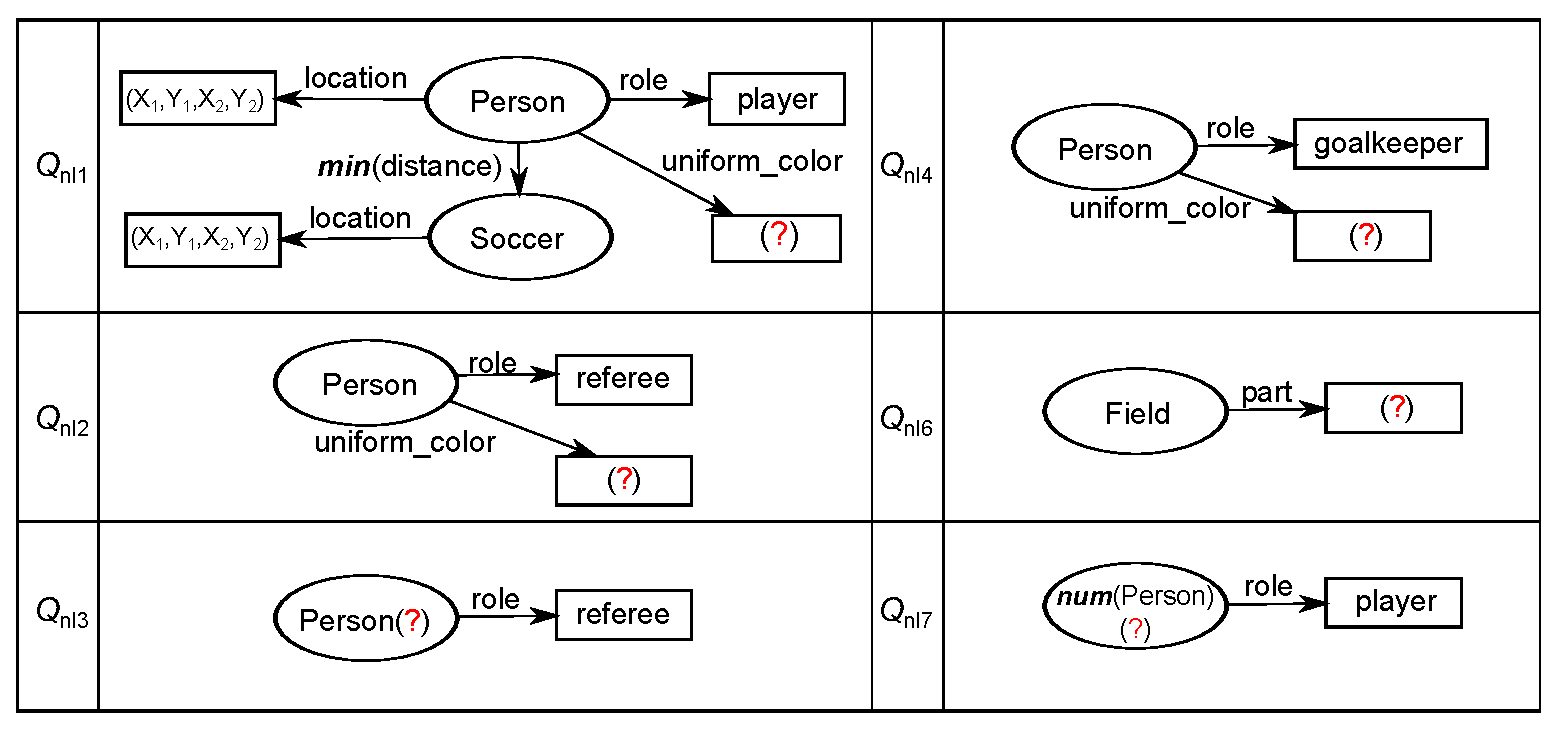
\includegraphics[width=\columnwidth]{queries.eps}
%\caption{Query graphs}
%\label{fig:queries}
%\end{figure}